\chapter{Obtaining the Data}
\label{chapter:obtainingData}
To train the models, as proposed in the previous chapters, and to validate their ranking qualities, data has to be obtained beforehand. We also need to know what metadata will be available before specifying global and attribute distances. Therefore, we need to gather datasets, metafeatures of those datasets, machine learning algorithms and experiment results prior to conducting the experiments with the ranking algorithms. The potential sources of such data and what metafeatures to use is the topic of this chapter. We will begin by defining the common format for storing datasets. Then we will discuss machine learning repositories and discuss their pros and cons. The differences lie mainly in the types of data available. We will discuss one particular machine learning repository -- OpenML -- in more details as it will be used as the main datasource. We then describe the dump we downloaded from the OpenML, filters we used to clean the dump, and the total amount of data we had after the filtering. This will include the decision to perform the ranking on the classification algorithms, therefore including the filter on classification tasks and algorithms only. We list the global metadata provided by the OpenML and discuss the subset that will be used for the experiments. As OpenML does not provide attribute metadata, we then review the types of attribute metadata we extracted. We look into the distribution of attribute metatadata in more detail and identify few potential problems in the distribution of attribute metadata. To tackle them, we introduce another attribute metafeatures that are calculated based on the previous metadata but do not suffer from the same problems.

\section{ARFF Format}
\label{section:arff}
In Section \ref{section:datasets}, we introduced the concept of datasets as a relation. That was however a mere theoretical description. The specification of mapping this theoretical description to a file is still needed. In this section, we describe the popular format called \emph{ARFF} (Attribute-Relation File Format) for storing datasets and therefore also classification and regression tasks. Its importance lies in that almost every machine learning tool and library supports ARFF and large amount of public datasets is distributed using this very format.

ARFF is a file format usually recognizable by the ".arff" file extension. 
An ARFF file is an ASCII text file that describes a list of instances sharing a set of attributes \cite{arff}. The file consists of two sections. The first one -- called Header -- contains descriptions, name of the relation and the list of attributes and their types. Description lines start with "\%" and can contain arbitrary information. 

The relation name is defined as the first line in the ARFF file. The format is: 
"@relation \$relation-name",
where \$relation-name is a string. The string must be quoted if the name includes spaces. 
The format for the @attribute statement is:
"@attribute \$attribute-name \$datatype",
where the \$attribute-name must start with an alphabetic character. If spaces are to be included in the name, then the entire name must be quoted.

The \$datatype can be any of the following:
\begin{itemize}
	\item numeric
	\item integer
	\item nominal
	\item string
	\item date
\end{itemize}
The header can contain arbitrary number of attributes.

The second section -- called Data --  starts with the @data declaration on a single line followed by lines of instances -- one data instance per line. Every instance consists of the list of values of the attributes in the same order. Missing values are encoded by "?".

The example of the ARFF format describes header and few instances of the Iris dataset \cite{iris} and is as follows: 
\begin{shaded}
	\noindent \% 1. Title: Iris Plants Database \\
	\% \\
	\% 2. Sources: \\
	\%      (a) Creator: R.A. Fisher \\
	\%      (b) Donor: Michael Marshall (MARSHALL\%PLU@io.arc.nasa.gov) \\
	\%      (c) Date: July, 1988 \\
	\% \\
	@RELATION iris \\
	\\
	@ATTRIBUTE sepallength  NUMERIC \\
	@ATTRIBUTE sepalwidth   NUMERIC \\
	@ATTRIBUTE petallength  NUMERIC \\
	@ATTRIBUTE petalwidth   NUMERIC \\
	@ATTRIBUTE class        {Iris-setosa,Iris-versicolor,Iris-virginica} \\
	\\
	@DATA \\
	5.1,3.5,1.4,0.2,Iris-setosa \\
	4.9,3.0,1.4,0.2,Iris-setosa \\
	4.7,3.2,1.3,0.2,Iris-setosa \\
	4.6,3.1,1.5,0.2,Iris-setosa \\
	5.0,3.6,1.4,0.2,Iris-setosa \\
	5.4,3.9,1.7,0.4,Iris-setosa \\
	4.6,3.4,1.4,0.3,Iris-setosa \\
	5.0,3.4,1.5,0.2,Iris-setosa \\
	4.4,2.9,1.4,0.2,Iris-setosa \\
	4.9,3.1,1.5,0.1,Iris-setosa 
\end{shaded}

All declarations are case insensitive.

The advantage of this file format is its simplicity. No special tools or libraries are required to parse ARFF files. This advantage inevitably comes with a big disadvantage -- there is no guarantee that the information stored in the file is consistent, especially entries stored in the Header section are often corrupted, or do not follow the format completely. 

\section{Machine Learning Repositories}
In this section, we discuss machine learning repositories that provide machine learning capabilities that may include datasets, algorithms, results and metadata. Therefore they make ideal candidates for the potential source of data for conducting machine learning experiments.

In the past, perhaps the most popular machine learning repository was the repository of University of California, Irvine abbreviated only as UCI \cite{uci}. The sole purpose of the repository was to provide public datasets (mostly in the ARFF format) for machine learning and metalearning experiments. Many works reviewed in this thesis used UCI as the source of data (including some of our works). The major drawback is that the repository does not provide any additional data besides datasets. Even if we used the UCI repository for datasets, additional data would still be needed. In our previous experiments, we combined the repository with our recommendation system Pikater (see Section \ref{section:recommenderSystems}) to gather the rest of the data. We used the search agents in Pikater for hyperparameter tuning of machine learning algorithms over UCI datasets. This resulted in a huge database containing 600,000 machine learning experiments results, which we used for our previous experiments with metalearning \cite{SSCI2014}. The purpose of building such experiments results was mainly in finding the best settings of hyperparameters for some machine learning algorithm on some datasets. Therefore, in terms of datasets, only 85 unique UCI datasets and 8 WEKA models were in these 600,000 results. This is a common phenomenon. Despite the fact that many machine learning experiments are conducted every day, the number of public datasets used for the experiments is small. We wanted to conduct the experiments in the thesis on the bigger dataset. One option was to use the system to create another batch of experiments.

Another option was to use the OpenML \cite{openMl} machine learning repository that emerged in the recent years. It is a repository of datasets, tasks, machine learning algorithms, and experiment results called runs. Most of UCI datasets are already present in OpenML, although many more datasets are also in the repository. OpenML user can also specify whether the dataset is private or public, however major number of datasets is public. When a new dataset is uploaded to a repository, OpenML automatically extracts metafeatures. There are in total 106 different metafeatures that can be extracted, however not every metafeature is extracted for each dataset. An OpenML task defines experiment over some dataset. It specifies the goal (e.g. supervised classification over the target attribute), estimation procedure (e.g. 10-fold cross-validation) and evaluation measures used (RMSE, PredictiveAccuracy). An OpenML run is the result of some machine learning algorithm on some task. 

As the experiment results are standardized, it is easy for researchers to compare the results of machine learning and metalearning methods. Furthermore, as some metafeatures are automatically computed by OpenML, it makes implementation of other metalearning approaches faster, thus speeding up the research. OpenML also exposes data via its REST API. Specialized connector packages for communication with this interface are available for R, Java, .Net (which was created by us) and Python. However, it is possible to write a custom connector, as almost all languages support REST API. Another benefit is that the whole project is under active development and there is a growing community around it. 

Not even  OpenML is without drawbacks. All datasets are visible including the testing data. With many experiments, there is no guarantee that users will not eventually carry information out of testing datasets into the training by looking at the results of previous experiments on the testing datasets (the phenomenon referred to as \emph{peeking} by authors of \cite{aima3ed}). The potential solution can be the gamification used for example in the \emph{Kaggle} site \cite{kaggle}. The testing dataset is not available and researchers have only a limited amount of time or submissions to submit their models. Therefore, the model cannot be built infinitely to reach the best testing result.

With the pros and cons in mind, OpenML was chosen as the source of data mainly because of its public availability, many experiments and datasets including those from UCI and global metadata autocomputed by the repository.
 
 The choice of the data is very important for the quality of experiments. Results can be affected by many factors -- amount of errors in the data, whether the data are general or domain specific only, etc. It should be taken into consideration that OpenML repository is very general and public. Therefore, it may contain errors or noise, and our algorithms have to handle every type of dataset.

\section{OpenML Dump}
\label{section:openMLDump}
In the previous section, we discussed the potential source of data and have chosen OpenML as the main data source.
Originally, our OpenML dump contained 791 public datasets. We have placed extra requirements on the datasets in order to fulfil following two requirements:
\begin{itemize}
	\item Keep the computation of alignment reasonable for all pairs of datasets in the chosen subset. This will speed up the evaluation of quality of alignment predictor. The computation cost depends on the number of attributes, the goal is to find a good compromise between the amount of datasets that we can use and the cost of alignment of their attributes.
	
	\item In order to be able to easily compare metalearning approaches, it is desirable that every dataset has the same types of metafeatures extracted. This may not be possible in every case, as some global metafeatures are only computable for classification/regression tasks. Because of this, some compromises may be needed. Similarly, some attribute metafeatures may be computable only for classification/numerical attributes but this does not concern us too much, as we will be using selectors (see Algorithm \ref{algo:combinedAlignmentHungarian}) to handle different types of attributes).
\end{itemize}
To find out the optimal compromise between the amount of datasets and attributes, we have plotted the distribution of number of attributes among datasets. The distribution is shown in Figure \ref{fig:numberOfAttributesDistribution}. It should be clear from the figure that only a very small number of datasets have large number of attributes. The alignment of this minority of datasets would take the majority of time. We have decided to filter the datasets with more than 50 attributes.

\begin{figure}
	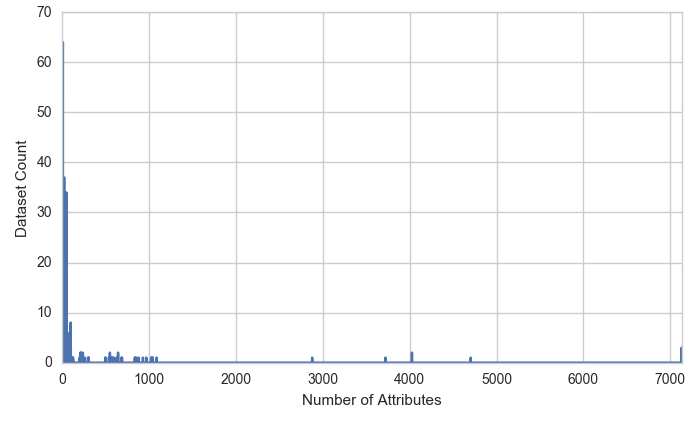
\includegraphics[width=14cm]{Images/numberOfAttributesDistribution.png}
	\centering
	\caption{Distribution of number of attributes among datasets in the OpenML dump.}
	\label{fig:numberOfAttributesDistribution}	
\end{figure}

The remaining datasets were examined for the distribution of the OpenML global metafeatures. The distribution is shown in Figure \ref{fig:globalmetadatadistirbution}. Not all global metafeatures are computed for each dataset. Luckily for us, in this case few metafeatures have useful property ensuring that if this metafeature was computed, then all others are computed (example of such metafeature was  kNN\_3NKappa). To fulfil the second criterion, it was then sufficient enough just to create a filter that one of these metafeatures cannot be null. After application of this filter, only classification datasets remained.

\begin{figure}
	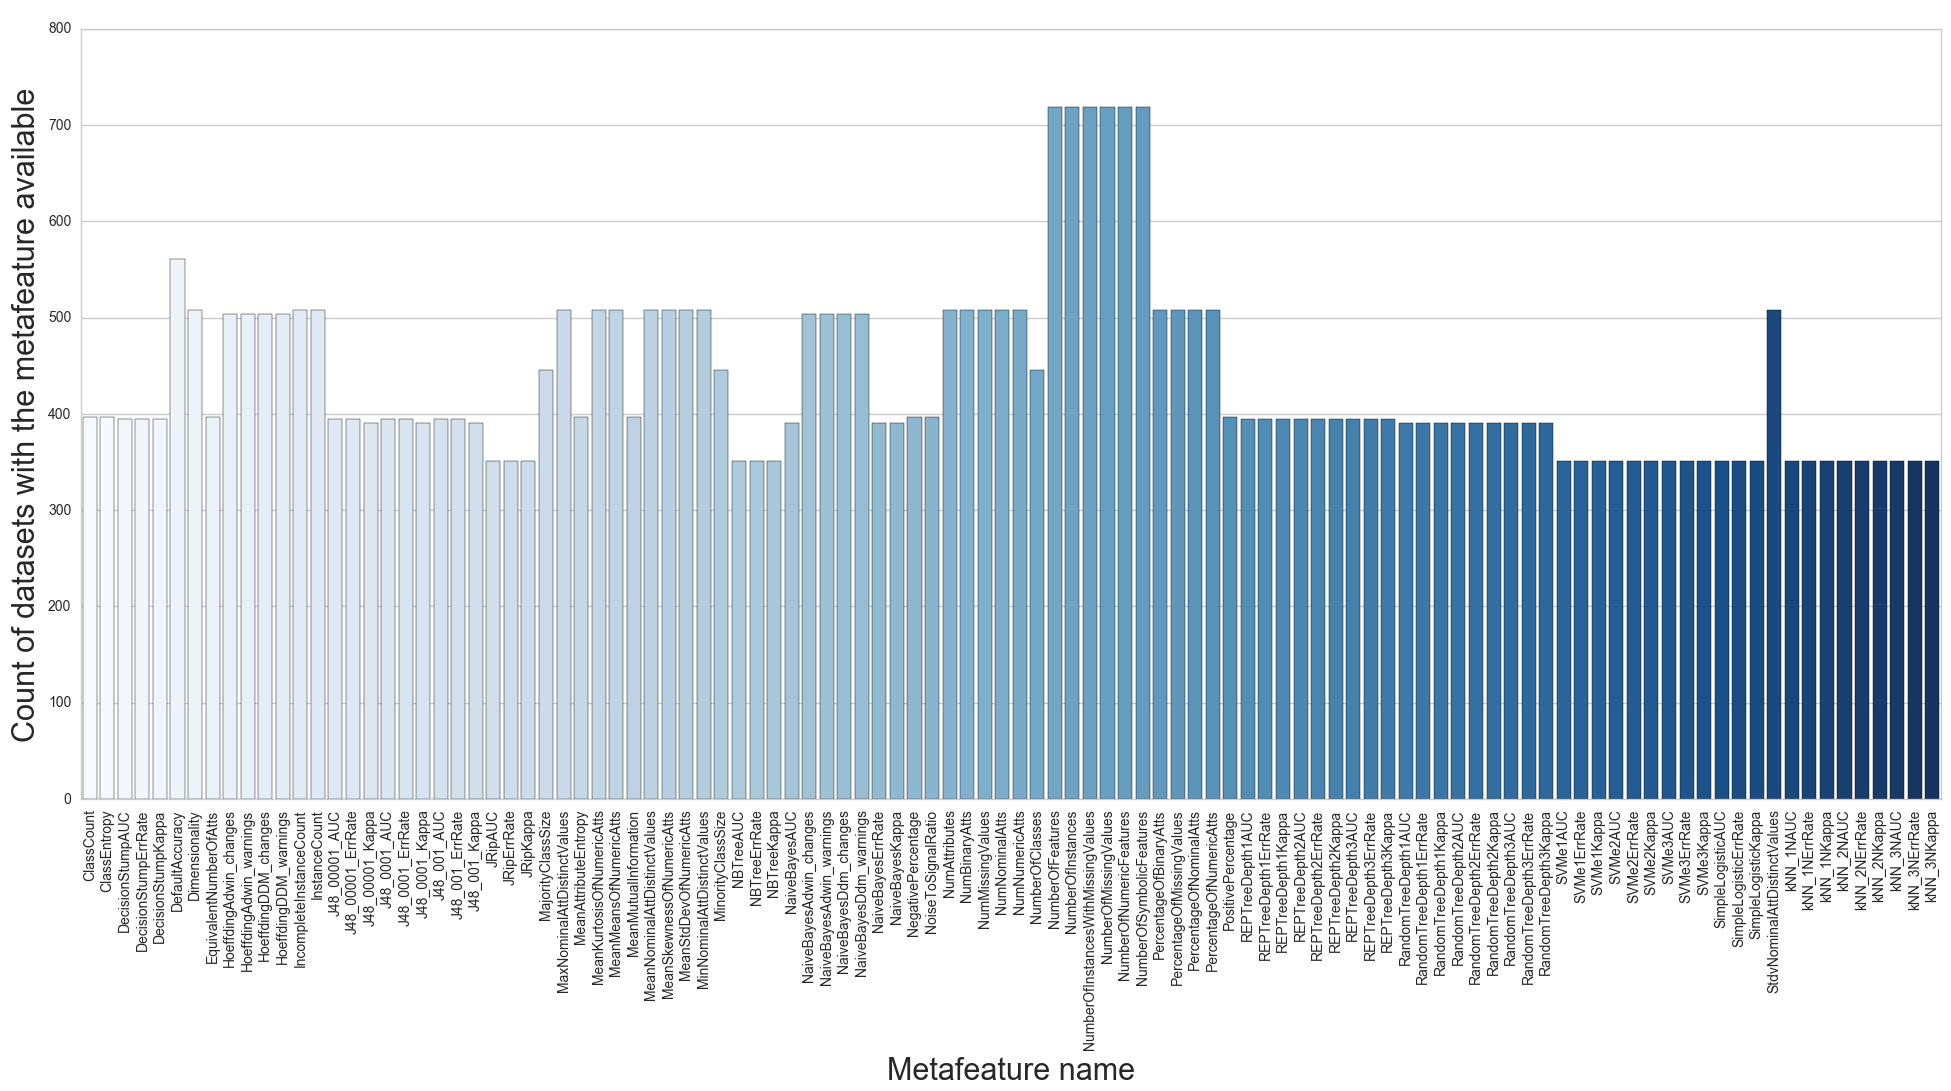
\includegraphics[width=14cm]{Images/OpenMlDataDistributtion.png}
	\centering
	\caption{Distribution of global metafeatures computed by OpenML.}
	\label{fig:globalmetadatadistirbution}	
\end{figure}

This data preprocessing included only dataset specific view. However, in our experiments the experiment results are also needed, which -- in the case of OpenML -- are covered by OpenML tasks and runs. First requirement was clear -- we can include only those datasets with the results available. Before stating another requirements, we have to choose some sort of performance criterion that will be used. We have already made the choice of restricting the datasets to classification datasets only. There are lots of performance measures possible for the classification task. When choosing a suitable measure, we wanted to include the criterion that is often used. This would minimize the filtering of datasets as this performance measure will be often available for each classification task. Based on this reasoning, we have chosen  Predictive Accuracy (see Definition \ref{definition:predictiveAccuracy}). There could still be multiple classification tasks defined with Predictive Accuracy as the performance measure -- they could still differ in the estimation procedure (simple training/testing split of the dataset, cross-validation, etc.). In order not to filter the data further, we have decided to neglect this difference, as the performance indicator is well defined regardless of the estimation procedure. Given the above, we can state the second requirement: we will include only those datasets that have some experiments results available with the Predictive Accuracy as one of the evaluation measures. 

There could be multiple results for a pair of algorithm, dataset. The question was which result to choose when arguing about the actual ranking of the algorithms on datasets. We argued that we want to asses the maximal potential of some algorithm. The best result also usually corresponds with a solution found by a hyper-parameter optimizer. Therefore, we have used the result with the best Predictive Accuracy.
 	
Finally, the results of ensemble algorithms like bagging, boosting, stacking and rotation forests \cite{rotationForests} were omitted. These ensembles are encompassing different number of other machine algorithms and can take advantage of such combined power. Such composite behaviour resulted in heavily outperforming every other algorithm in the database, thus changing the results significantly. Furthermore, their performance relies heavily on the parameters that specify what algorithms should be used in the ensemble and as such, every parameter setting should be better treated as a separate algorithm. More careful examination is thus necessary before including ensemble algorithms into our experiments.

Application of the filters resulted in 351 datasets with 20,719 rows of the best results with Predictive Accuracy for some pair of algorithm and dataset. That included 115 unique algorithms.

These amounts may seem low for machine learning experiments, but they are still much bigger that in our previous experiments, and are very high also compared to the rest of the metalearning experiments found in the literature.

Unfortunately, not every algorithm was run over every dataset. Therefore, results of some algorithms did not have to appear in the neighbourhood considered by the $k$-NN algorithm. We decided to calculate the ranking only for the algorithms that were available in the neighbourhood. This could affect the quality of ranking evaluation, however, such negative consequences can be minimized by choosing high enough $k,$ so the neighbourhood is more likely to contain more algorithms. Furthermore, high values returned by ranking quality evaluator still means high quality ranking, although not on every dataset. This can be seen as a noise or as missing values presented in the data.

The final question was splitting the data into the training and testing datasets. As the space was not very dense, and the $k$-NN that we were going to use is very dependent on the space density, we decided to split the datasets with 1:1 ratio. This enabled better estimation of the overfitting. If we used a different ratio, even the model with good generalization abilities could have much different results on the testing dataset, because of the space with much different density.

\section{Metadata}
This section will discuss which metadata were available or computed. First, we are going to discuss global data. Second, attribute metadata are described. This section also discusses normalization of both the global and attribute metadata. Note that different algorithms use different metadata, this will be elaborated when discussing experiment details.

\subsection{Global Metadata}
 As discussed in the previous section, we have filtered the OpenML dump in such a way that every metadata is available for each dataset. 
 We have argued whether we should include all the types of global metadata or just the simple, statistical, and information-theoretic ones. There are two reasons for this. First, we will base the attribute metafeatures on the simple, statistical, and information-theoretic types. Including the model based and landmarker features would make it harder to see whether the aggregation of attribute metafeatures indeed lose important information. Second reason is that model based and landmarkers metafeatures can contain information about performance on the the training and testing set. We would have to filter the training and testing set for such use to mitigate this risk. For these reasons, we have decided to use only the simple, statistical, and information-theoretic global metafeatures. In the production use, we would however include metadata of every type.
 
OpenML machine learning repository contained the following simple, statistic, and information theoretic global metadata:
\begin{itemize}
	\item ClassEntropy -- entropy of the target attribute.
	\item DefaultAccuracy -- default accuracy obtained by the baseline algorithm. In this case by predicting always the majority class. 
	\item Dimensionality -- number of attributes divided by the number of instances.
	\item InstanceCount -- number of instances (rows) of the dataset.
	\item MajorityClassSize -- number of instances with the most frequent class of the target attribute.
	\item MaxNominalAttDistinctValues -- the maximum number of distinct values among attributes of the nominal type.
	\item MinNominalAttDistinctValues -- the minimal number of distinct values among attributes of the nominal type.
	\item MinorityClassSize -- number of instances with the least frequent class of the target attribute.
	\item NumAttributes -- number of attributes (columns) of the dataset.
	\item NumBinaryAtts -- count of binary attributes.
	\item NumNominalAtts -- count of nominal attributes.
	\item NumNumericAtts --  count of categorical attributes.
	\item PercentageOfBinaryAtts -- percentage of binary attributes.
	\item PercentageOfNominalAtts -- percentage of nominal attributes.
	\item PercentageOfNumericAtts -- percentage of numerical attributes.		
	\item NumberOfClasses --  number of classes for the classification task.
	\item IncompleteInstanceCount -- number of instances with at least one value missing.
	\item NumMissingValues -- number of missing values in the dataset.
	\item PercentageOfMissingValues -- percentage of missing values.
	\item PositivePercentage -- percentage of rows with the class with the highest assigned index. In the case of binary classification this is equal to percentage of positive instances.
	\item NegativePercentage -- percentage of rows with the class with the lowest assigned index. In the case of binary classification this is equal to percentage of negative instances.	
	\item MeanAttributeEntropy -- mean of entropy among attributes.
	\item MeanKurtosisOfNumericAtts -- mean kurtosis among attributes of the numeric type.
	\item MeanMeansOfNumericAtts -- mean of means among attributes of the numeric type.
	\item MeanMutualInformation -- mean of mutual information between the nominal attributes and the target attribute.
	\item MeanNominalAttDistinctValues -- mean of number of distinct values among the attributes of the nominal type.
	\item MeanSkewnessOfNumericAtts -- mean skewness among attributes of the numeric type.
	\item MeanStdDevOfNumericAtts -- mean standard deviation of attributes of the numeric type.
	\item NoiseToSignalRatio -- ClassEntropy divided by MeanMutualInformation. Returns -1 if MeanMutualInformation is zero.
	\item EquivalentNumberOfAtts -- The difference of (MeanAttributeEntropy - MeanMutualInformation) divided by MeanMutualInformation. Returns -1 if MeanMutualInformation is zero.
	\item StdvNominalAttDistinctValues -- standard deviation of the number of distinct values among nominal attributes.
\end{itemize}

We have also identified some duplicates among the meatefatures: \\ NumberOfMissingValues as a~duplicate of NumMissingValues, ClassCount as a~duplicate of NumberOfClasses, NumberOfInstances as a~duplicate of InstanceCount, NumberOfFeatures as a~duplicate of NumAttributes, NumberOfNumericFeatures as a~duplicate of NumNumericAtts, NumberOfSymbolicFeatures as a~duplicate of NumNominalAtts and NumberOfInstancesWithMissingValues as a~duplicate of IncompleteInstanceCount metafeature. We have removed the duplicates out of a set of metafeatures used.

The last few attributes beginning with the MeanAttributeEntropy represent exactly those attributes where some important information may be lost during the aggregation, as discussed in Section \ref{section:NonpropositionalApproachToMetalearning}.

The excluded metadata (of model based or landmarker type) are listed in Table \ref{table:excludedGlobalMetadata}. We will omit their description, as they are no longer relevant.

 \begin{table} 
 	\caption{Excluded global metafeatures.}
 	\label{table:excludedGlobalMetadata}
 	\centering 
 	\renewcommand{\arraystretch}{1.3}
 	\begin{tabular}{|c| c| c|} 	
 		\hline 	 
	 	RandomTreeDepth1AUC & REPTreeDepth3AUC & J480001ErrRate \\
	 	RandomTreeDepth1ErrRate & REPTreeDepth3ErrRate & J48001ErrRate \\
	 	RandomTreeDepth1Kappa & REPTreeDepth3Kappa & JRipErrRate \\
	 	RandomTreeDepth2AUC & DecisionStumpAUC & NBTreeErrRate \\
	 	RandomTreeDepth2ErrRate & DecisionStumpErrRate & SVMe2ErrRate \\
	 	RandomTreeDepth2Kappa & DecisionStumpKappa & kNN1NErrRate \\
	 	RandomTreeDepth3AUC & SimpleLogisticAUC & NBTreeAUC \\
	 	RandomTreeDepth3ErrRate & SimpleLogisticErrRate &  kNN2NErrRate\\
	 	RandomTreeDepth3Kappa & SimpleLogisticKappa & J480001AUC \\
	    HoeffdingAdwinChanges & NaiveBayesAUC  & JRipKappa \\
	    HoeffdingAdwinWarnings & NaiveBayesErrRate & SVMe3ErrRate \\
	    HoeffdingDDMChanges & NaiveBayesKappa  & SVMe1AUC \\
	    HoeffdingDDMWarnings & SVMe1Kappa & SVMe2AUC \\
	    NaiveBayesAdwinChanges & SVMe2Kappa & SVMe3AUC \\
	    NaiveBayesAdwinWarnings & SVMe3Kappa & J48001AUC \\
	    NaiveBayesDdmChanges & kNN3NErrRate & kNN1NAUC \\
	    NaiveBayesDdmWarnings & kNN1NKappa & kNN2NAUC \\
    	REPTreeDepth1AUC & J480001Kappa &  J48001Kappa\\
    	REPTreeDepth1ErrRate & NBTreeKappa & SVMe1ErrRate \\
    	REPTreeDepth1Kappa & J4800001AUC & J4800001ErrRate \\
	    REPTreeDepth2AUC & kNN2NKappa & kNN3NAUC \\
   	    REPTreeDepth2ErrRate & JRipAUC &  J4800001Kappa\\
   	    REPTreeDepth2Kappa & kNN3NKappa & \\
 		\hline 
 	\end{tabular}
 \end{table}  

To sum up, we had 31 global metafeatures available for each dataset.

\subsection{Attribute Metadata}
There is no such public repository as OpenML that would have attribute metadata available for each dataset. Some information could be available in the header of the ARFF files (see Section \ref{section:arff}), but as already discussed, there is no guarantee that the information really corresponds to values in the data. Indeed, we have encountered datasets that were corrupted this way. Furthermore, this information is optional, thus not available in every header. Based on these facts, we decided to build our own ARFF analyser. The analyser was able to read the input ARFF file and extract various attribute metadata. In the rest of this section, we describe the attribute metafeatures extracted. As our algorithms are capable of handling type-specific attribute metadata using selectors (see Algorithm \ref{algo:combinedAlignmentHungarian}), we will list them according to the type of attribute they were extracted for.

In order to be able to compute some metafeatures for the categorical attributes, a conversion to the integers was made. Distinct number was assigned to each category. The number was chosen based on the order of appearance beginning with one.

Measures common for both the categorical and numerical metafeatures:
\begin{itemize}	
	\item ForRegression -- whether the target was of numerical type (this was not used as we have used only classification tasks).
	\item ValuesCount -- number of values.
	\item NonMissingValuesCount -- number of non missing values.
	\item MissingValuesCount -- number of missing values.
	\item Distinct -- number of distinct values (classed).
	\item AverageClassCount  -- average count of occurrences among different classes.
	\item Entropy -- entropy of the values.
	\item MostFequentClassCount -- count of the most probable class.
	\item LeastFequentClassCount  -- count of the least probable class.
	\item ModeClassCount -- mode of the number of distinct values.
	\item MedianClassCount -- median of the number of distinct values.
	\item PearsonCorrellationCoefficient -- Pearson Correlation Coeeficient of the values and the values of target attribute.
	\item SpearmanCorrelationCoefficient -- Spearman Correlation Coeeficient of the values and the values of target attribute.
	\item CovarianceWithTarget -- covariance of the values with the values of the target attribute.
\end{itemize}

Numerical metadata:
\begin{itemize}	
	\item IsUniform -- whether statistical test did not reject that the attribute values corresponds to a uniform distribution.   
	\item IntegersOnly -- whether attribute values contained only integers.    
	\item Min -- minimal value of the attribute values.
	\item Max  -- maximal value of the attribute values.
	\item Kurtosis -- kurtosis of the values.
	\item Mean -- mean of the values.
	\item Skewness -- skewness of the values.
	\item StandardDeviation -- standard deviation of the values.
	\item Variance -- variance of the values.   
	\item Mode -- mode of the values.   
	\item Median -- median of the values.  
	\item ValueRange -- difference between maximum and minimum of the values.  
	\item LowerOuterFence -- lower outer fence of the values.  
	\item HigherOuterFence -- higher outer fence of the values.  
	\item LowerQuartile  -- lower quartile.  
	\item HigherQuartile -- higher quartile of the values.   
	\item HigherConfidence -- higher confidence interval of the values.  
	\item LowerConfidence -- lower confidence interval of the values.      
	\item PositiveCount -- number of positive values.   
	\item NegativeCount -- number of negative values.   
	
\end{itemize}

Categorical metadata:

\begin{itemize}	
	\item Uniform Discrete -- result of Pearson's chi-squared test for discrete uniform distribution.
	\item $\chi^2$ Statistic  -- statistic value for the Pearson's chi-squared test.
	\item Ratio of attribute values that after sub-setting the dataset to that attribute value lead to different distribution of the target as indicated by the following statistical test:
	\begin{itemize}
		\item Kolmogorov-Smirnoff test (continuous target only),
		\item Mann-Whitney U-test (continuous target only),
		\item $\chi^2$-test (categorical target only).
	\end{itemize}
\end{itemize}

To sum up, we have extracted 15 types of attribute metadata available for both the numerical and categorical attributes, another 20 types for numerical attributes and 3 types for categorical attributes only.

\subsection{Normalization}
Our algorithms were designed with no prior distinction of the metafeatures.
Some metafeatures put on much bigger values than the others. If we used the vector of constant weights, the $p$-norm distance could yield distance mainly derived out of big valued attributes. This would mitigate the influence of the attributes with small absolute values even though those could contain important information. To be precise, some metafeatures in our database have values as high as 445694751099523.38 ($variance$ metafeature) and as low as -142020048 ($minimum$ metafeature), other metafeatures have by definition values constrained to some interval (for example (Spearman's Correlation Coefficient with the range of $\langle -1,1 \rangle$).

For this reason, we have normalized most metafeatures into the interval $\langle 0,1 \rangle$. Attributes already naturally constrained to that or similar interval (Spearman's Correlation Coefficient) were the exception. The normalization was performed regardless of whether the metafeature was global or attribute specific. We have used the $min-max$ normalization given by the following equation:

\begin{equation*}
x'_i=\frac{x_i - \min_{x \in \mathbb{X}}}{\max_{x \in \mathbb{X}}-\min_{x \in \mathbb{X}}},
\end{equation*}
where $\min_{x \in \mathbb{X}}$ and $\min_{x \in \mathbb{X}}$ are minimal and maximal values of the given metafeature $\mathbb{X}$, $x_i$ is specific value of the $i$-th metafeature before rescaling, and $x'_i$ the value of that metafeature after rescaling.

This solved the original problem, but sometimes another problem emerged. In some cases the majority of values lied in some small subinterval of $\langle 0,1 \rangle$. Even when the metafeature had been assigned with high weight, the distance on this single metafeature would still be around zero between most of the metafeature values and very high between few outliers and the rest of the values. This would neglect the usefulness of such metafeatures including one that could be expected to bring high discriminative factor into the distinguishing of attributes, such as maximum and minimum values.

The box plots after min-max normalization are plotted for categorical metafeatures in Figure \ref{fig:categoricalAttributeDistribution} and  for the numerical attributes in Figure \ref{fig:numericalAttributeDistribution}.
The metafeatures suffering from such problem are those whose boxplot is small compared to the interval. In some cases, the boxplot quartiles are blending together and such cases are the most problematic ones. 
To partially mitigate the problem, we have introduced virtual metafeatures, that means metafeatures computed given different features that were independent of the values and size of the dataset - percentage or boolean values calculated out of metafeatures. Percentage or boolean are naturally normalized between $\langle 0,1 \rangle$ and should not have some outliers as in the case of metafeatures based on counts. The virtual metafeatures added were the following:

Measures common for both the categorical and numerical metafeatures:
\begin{itemize}
	\item MissingValues -- Boolean whether count of missing values is greater than 0.
	\item AveragePercentageOfClass -- Percentage of the occurrences among classes, calculated by AverageClassCount/Values count.
	\item PercentageOfMissing -- Percentage of missing values in the attribute, calculated by MissingValuesCount/Values count.
	\item PercentageOfNonMissing -- Percentage of non missing values in the attribute, calculated by 1 - Percentage of missing.
	\item PercentageOfMostFrequentClass -- Percentage of the most frequent class calculated as Most Frequent Class Count/Values count. 
	\item PercentageOfLeastFrequentClass -- Percentage of the least frequent class calculated as Least Frequent Class Count/Values count. 
	\item ModeClassPercentage -- Percentage of mode of class count calculated as Mode Frequent Class Count / Values count.
	\item MedianClassPercentage -- Percentage of median of class count calculated as Median Frequent Class Count / Values count.	
\end{itemize}

Numerical metafeatures:
\begin{itemize}
	\item PositivePercentage -- Percentage of positive values calculated as $\frac{PositiveCount}{ValuesCount}$.
	\item NegativePercentage -- Percentage of negative values calculated as $\frac{NegativeCount}{ValuesCount}$.  
	\item HasPositiveValues -- Boolean whether attribute values contain positive values. Determined as the result of $PositiveCount > 0$.
	\item HasNegativeValues -- Boolean whether attribute values contain negative values. Determined as the result of $NegativeCount > 0$.
\end{itemize}

Adding the virtual attributes does not mean that the rest of the problematic features should be thrown away. They could still be valuable for detecting outliers in the data, thus useful for identifying distant attributes (or datasets).

In total we have added 8 virtual metafeatures available regardless of attribute type and 4 virtual attributes for the numerical attributes. With the number of original attributes, it made 23 attributes for all types, 24 for numerical attributes, and additional 3 for categorical attributes.

\begin{figure}
	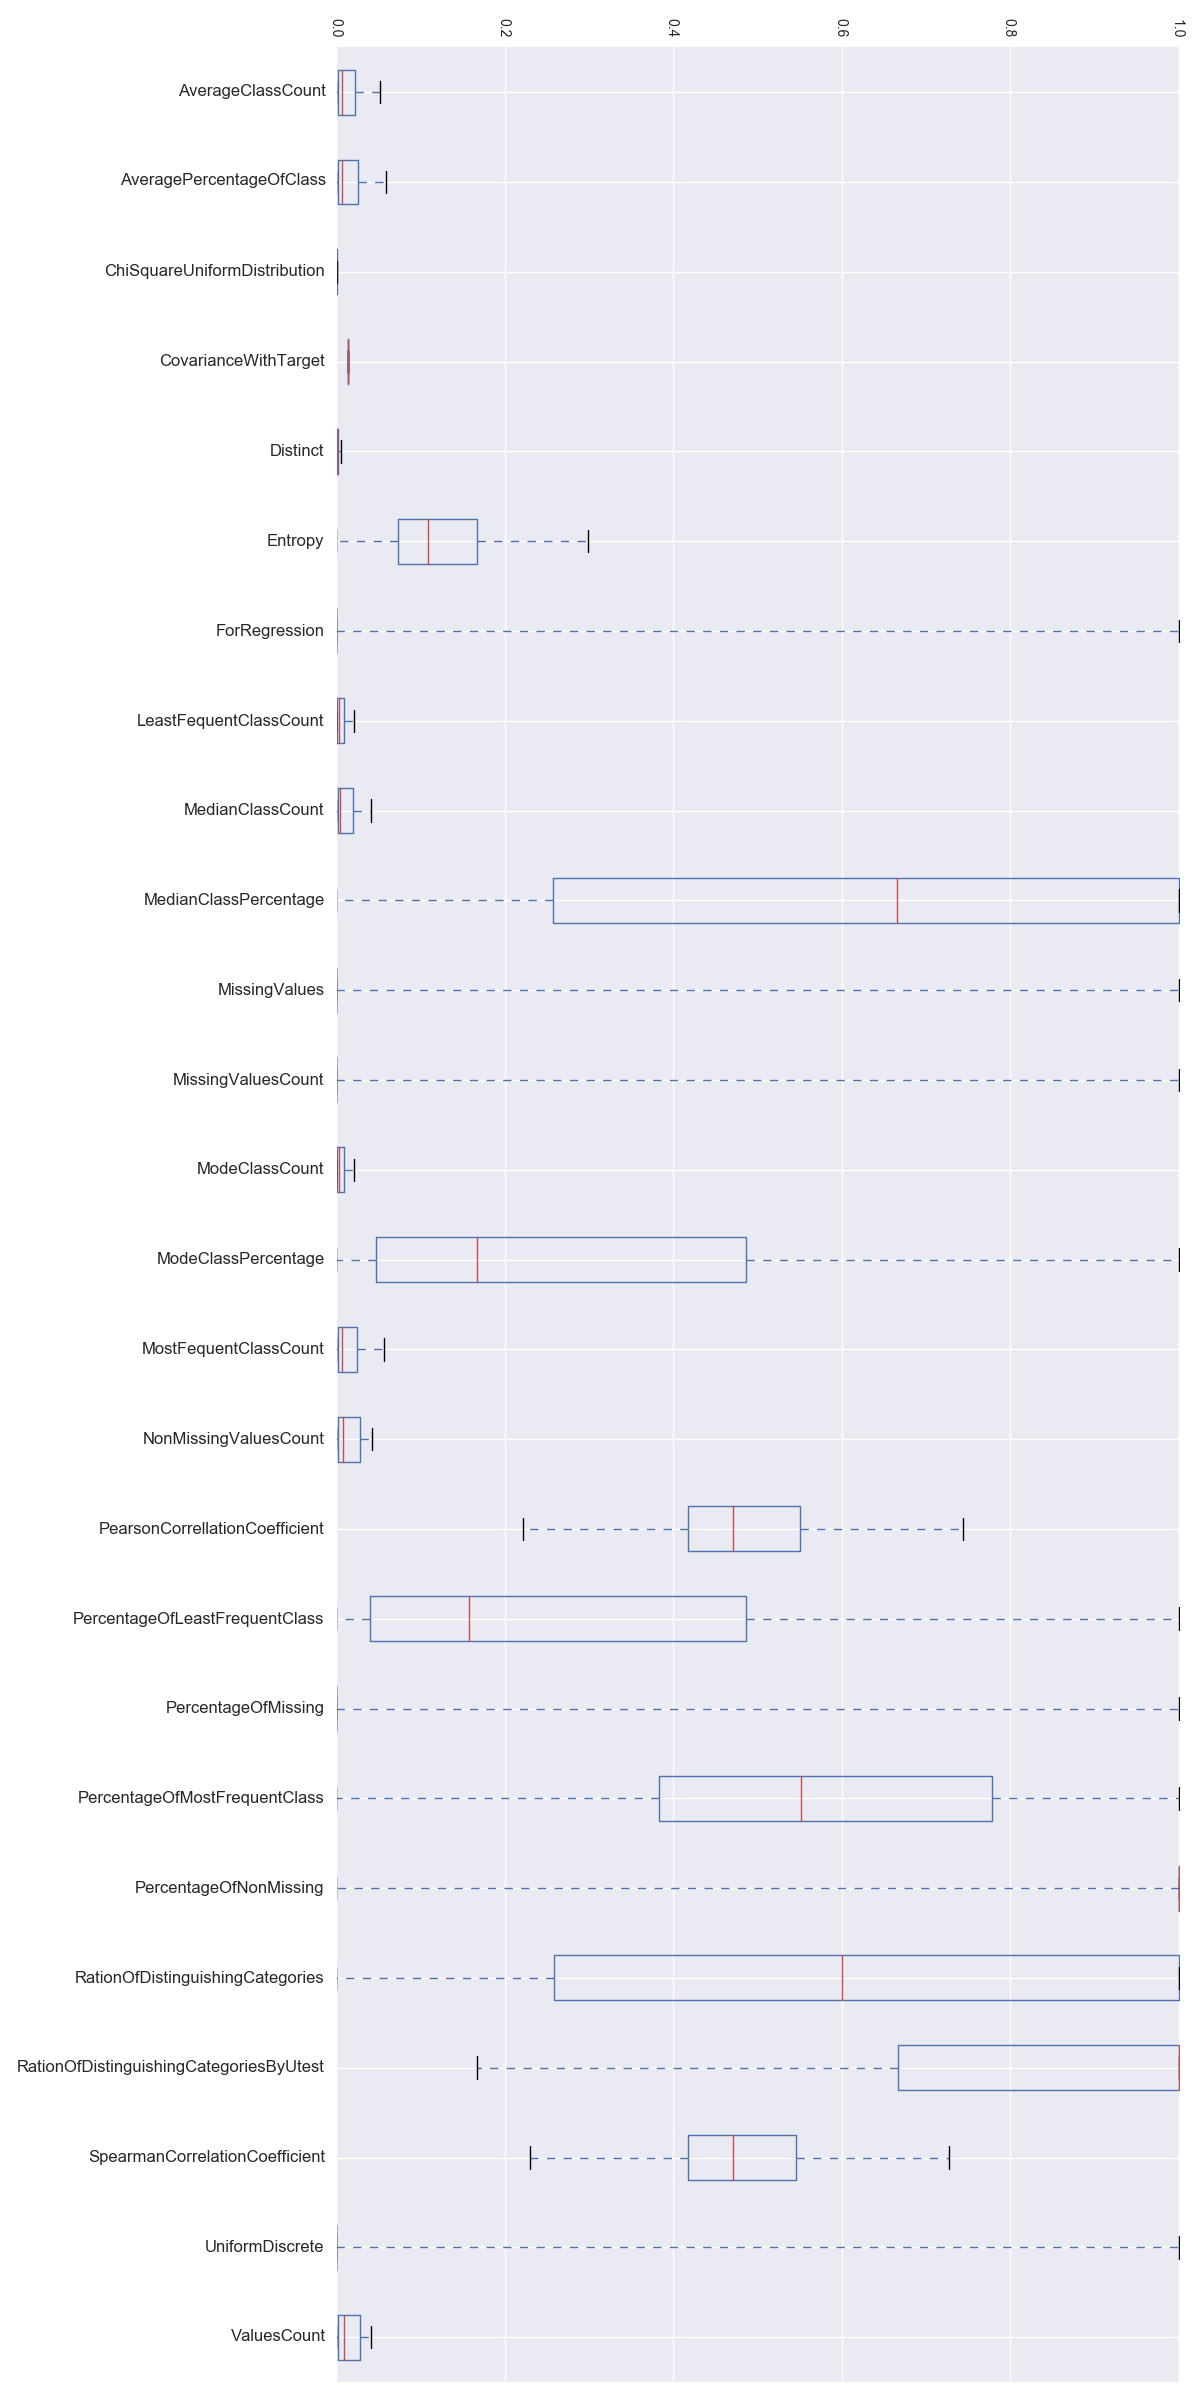
\includegraphics[width=12cm]{Images/categoricalAttributeDistribution.png}
	\centering
	\caption{Distribution of values of categorical metafeatures after normalization.}
	\label{fig:categoricalAttributeDistribution}	
\end{figure}

\begin{figure}
	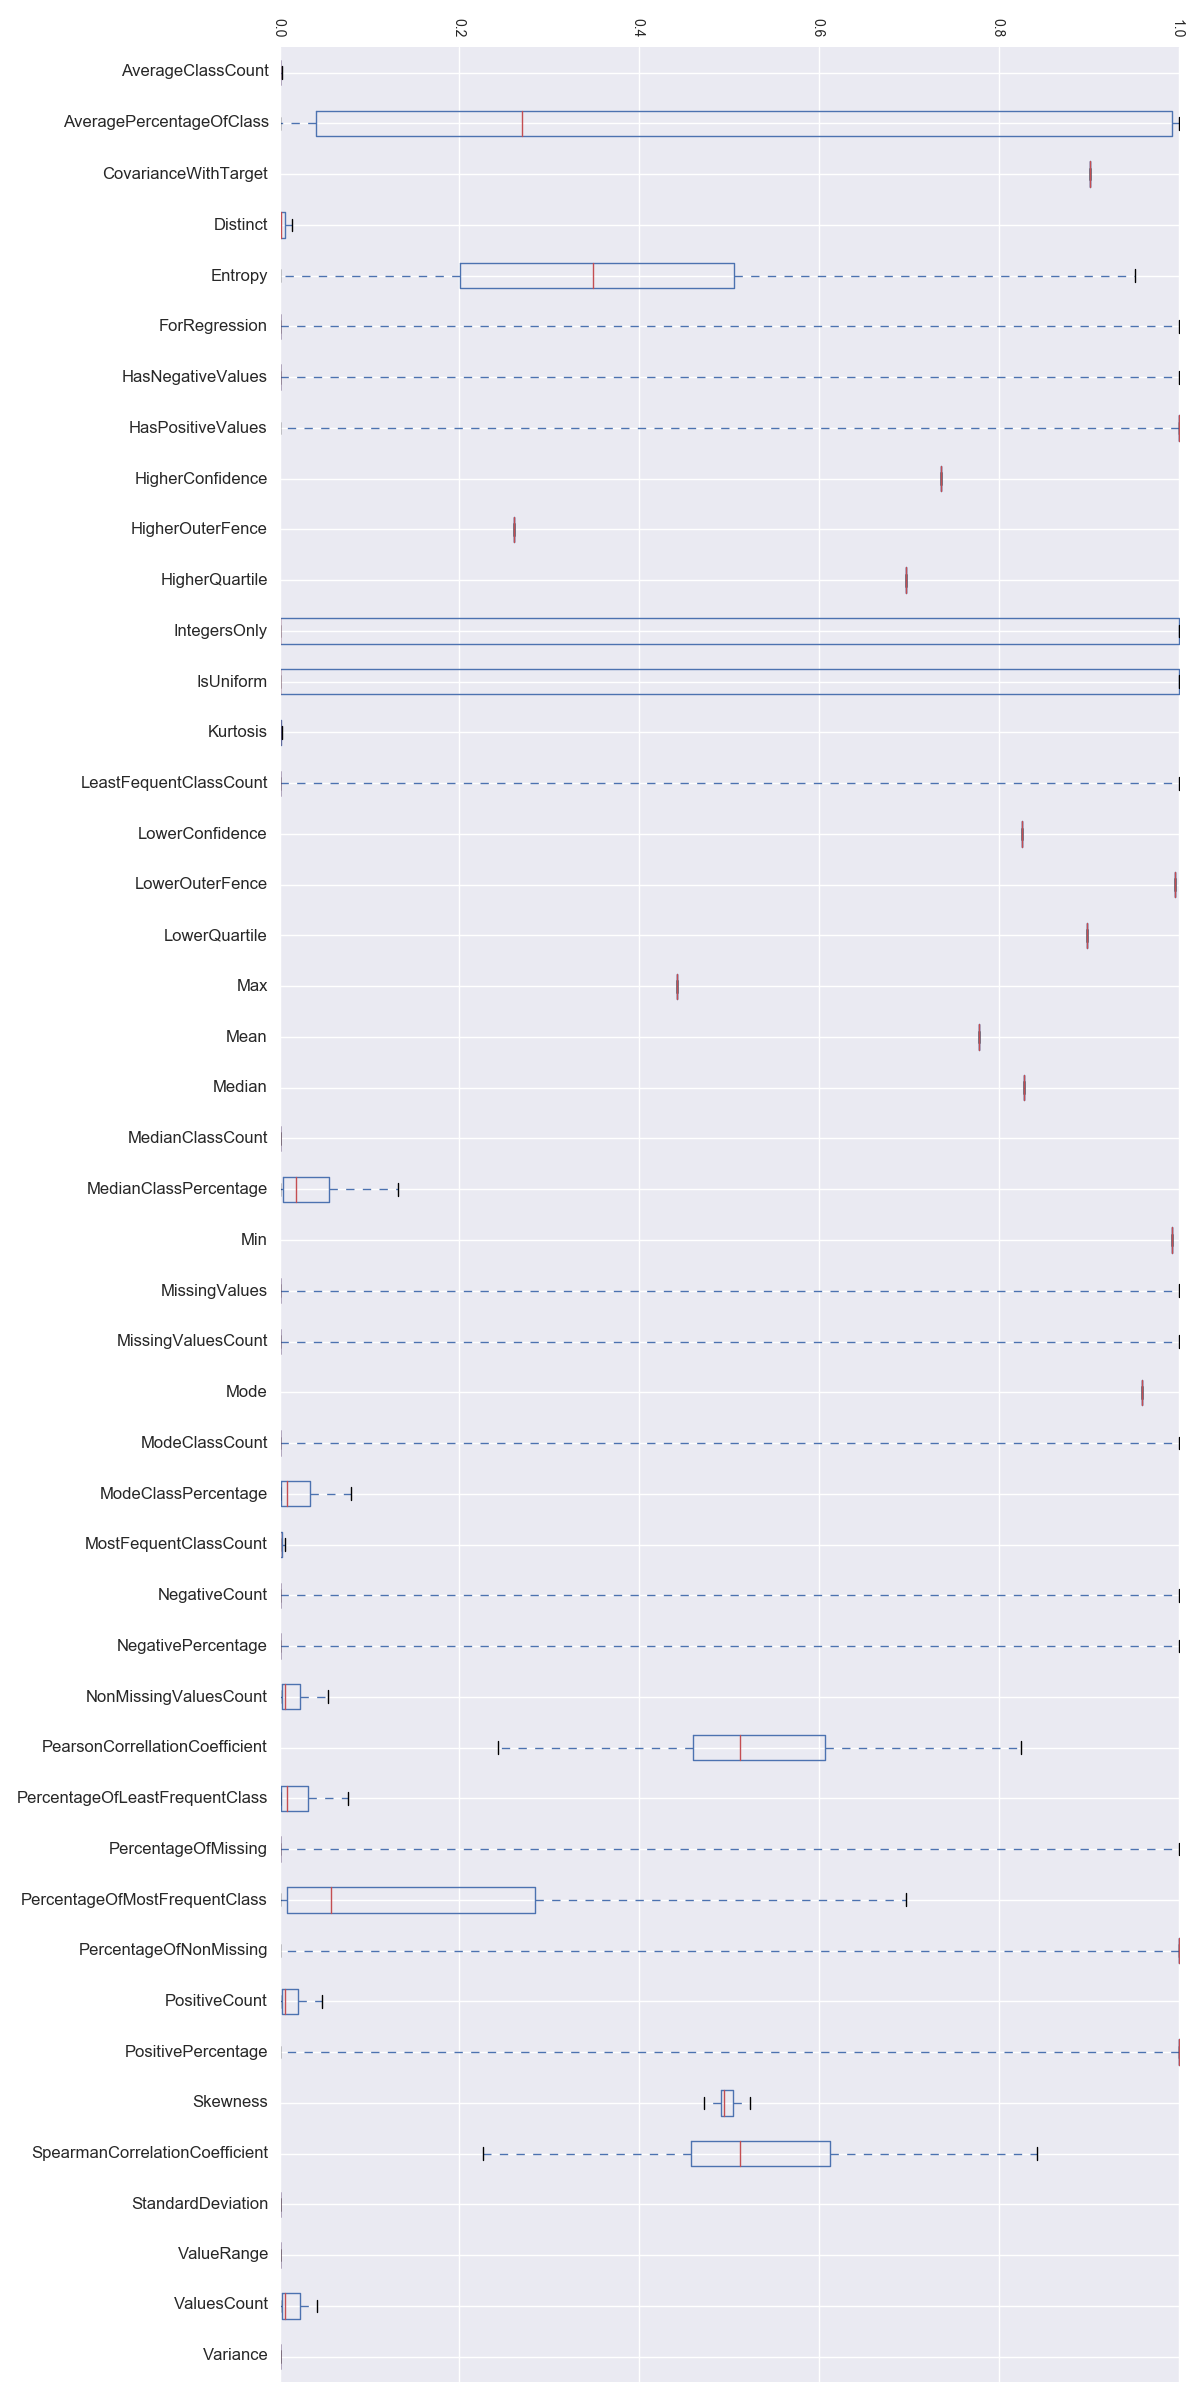
\includegraphics[width=12cm]{Images/numericalAttributeDistribution.png}
	\centering
	\caption{Distribution of values of numerical metafeatures after normalization.}
	\label{fig:numericalAttributeDistribution}	
\end{figure}
 

 